\documentclass[12pt]{article}
\usepackage[a4paper, total={6in, 8in}]{geometry}
\usepackage{graphicx}
\usepackage{amsmath}
\usepackage[utf8]{inputenc}
\usepackage[hidelinks]{hyperref}
\hypersetup{
    colorlinks=true,
    linkcolor=blue,      % Internal links
    urlcolor=blue,       % External links
    citecolor=blue       % Color of citations
}
\usepackage[T1]{fontenc}

\title{\textbf{EV MASTER CLASS CAPSTONE PROJECT}}
\author{}
\date{}

\begin{document}

\maketitle

\begin{center}
    \Large \textbf{Simulation of On-Board Charger for E-Bike Application}
\end{center}

\section*{Author Information}
\begin{itemize}
    \item \textbf{Name}: Pragya Sujitkumar
    \item \textbf{Email}: \href{mailto:pragyasujitkumar922004@gmail.com}{pragyasujitkumar922004@gmail.com}
    \item \textbf{Phone Number}: +91 9611553678
    \item \textbf{Institute}: Manipal Institute of Technology, Manipal
    \\
    \item \textbf{Name}: Srikar Bharadwaj R
    \item \textbf{Email}: \href{mailto:srikarbharadwaj000@gmail.com}{srikarbharadwaj000@gmail.com}
    \item \textbf{Phone Number}: +91 7259595751
    \item \textbf{Institute}: Manipal Institute of Technology, Manipal
\end{itemize}

\newpage

\section*{eBike Onboard Charger Design - Assumptions}

The following parameters were selected to ensure compatibility and efficiency for typical eBike battery requirements.

\section*{Design Assumptions}
The onboard charger was designed with the following key parameters:

\subsection*{1. Input Voltage (Vin): 110-240V AC}
\begin{itemize}
    \item \textbf{Range:} The charger is compatible with standard AC wall outlets across a wide voltage range, from 110V to 240V.
\end{itemize}

\subsection*{2. Output Voltage (Vout): 48V DC}
\begin{itemize}
    \item \textbf{Battery Compatibility:} The 48V DC output is tailored to match the standard voltage requirements for most eBike battery packs.
    \item \textbf{Stable Output:} This voltage ensures the charger delivers a steady DC output compatible with the onboard battery management system (BMS).
\end{itemize}

\subsection*{3. Output Current (Iout): 5A}
\begin{itemize}
    \item \textbf{Safe Charging Rate:} An output current of 5A is optimized to charge eBike batteries effectively without overheating or overloading the cells.
    \item \textbf{Extended Battery Life:} This moderate current level minimizes stress on battery cells, supporting longer battery life by reducing the risk of overcurrent.
\end{itemize}

\subsection*{4. Output Power: 240W}
\begin{itemize}
    \item \textbf{Efficient Power Delivery:} With a total output power of 240W, the charger provides sufficient power for timely charging of most eBike battery sizes.
\end{itemize}

\subsection*{5. Charging Efficiency: >90\%}
\begin{itemize}
    \item \textbf{Energy Efficiency:} The charger is designed to achieve an efficiency of greater than 90\%, ensuring that most of the power drawn from the AC source is effectively transferred to the battery.
    \item \textbf{Reduced Heat Generation:} High efficiency minimizes power losses, leading to less heat generation during operation, which is crucial for maintaining safe temperatures in compact eBike chargers.
\end{itemize}

\section*{Full-Bridge Rectifier Circuit}
A \textbf{Full-Bridge Rectifier} is used to convert alternating current (AC) to direct current (DC) by using four diodes arranged in a bridge configuration. This circuit allows the current to always flow in the same direction, regardless of the AC polarity. It includes a capacitor to filter the output DC voltage and reduce ripple.

\subsection*{Components and Operation}

\begin{itemize}
    \item \textbf{Input AC Voltage (Vin)} \\
    The input is an AC voltage of 230V, 50Hz, which is supplied to the full-bridge rectifier. This AC voltage alternates its polarity at 50 cycles per second (50Hz).

    \item \textbf{Diodes} \\
    The four diodes in the full-bridge configuration allow current to flow in one direction during both half-cycles of the AC input, thereby converting the AC to pulsating DC. The diodes ensure that the output voltage is always positive, regardless of the polarity of the input AC.

    \item \textbf{Capacitor (C = 3.074mF)} \\
    A capacitor is placed in parallel with the output load to smooth out the pulsating DC voltage and reduce the ripple. This helps in providing a more stable DC output.

    \begin{itemize}
        \item \textbf{Capacitor Calculation}: \\
        The capacitance value is selected to reduce the ripple voltage to an acceptable level. The formula for calculating the required capacitance is:
        \[
        C = \frac{I_{\text{load}}}{2 \cdot f \cdot \Delta V}
        \]
        where:
        \begin{itemize}
            \item $C$ = Capacitance in Farads (F)
            \item $I_{\text{load}}$ = Load current in Amps (A)
            \item $f$ = Frequency of the input AC (in Hz), which is 50 Hz for this case
            \item $\Delta V$ = Ripple voltage (in Volts)
        \end{itemize}

        For instance, to filter the ripple effectively, a capacitor of \textbf{3.074 mF} is used, which can handle the load current and reduce the ripple to a minimal value.
        \end{itemize}

    \item \textbf{Resistive Load (R = 322$\Omega$)} \\
    The output of the rectifier is connected to a \textbf{resistive load} of 322$\Omega$. The current drawn by the load is determined by Ohm’s law:

    \[
    I = \frac{V_{\text{DC}}}{R}
    \]

    Given the output voltage of the rectifier is 230V RMS, it will be stepped up after rectification to a DC voltage of approximately \( V_{\text{DC}} = V_{\text{peak}} - V_{\text{diode drop}} \),

    where \( V_{\text{peak}} = \sqrt{2} \times 230V \).
\end{itemize}

  \subsection*{Buck Converter (Current = 0.8412A)}
    Replacing the resistive load with the previously mentioned \textbf{buck converter}, the load current is reduced to \textbf{0.8412A}. The output DC voltage from the rectifier remains steady at around \textbf{325V}, and the buck converter will step down this voltage to its desired level.

  \subsection*{Ripple Voltage Reduction}
    The capacitor (3.074mF) helps reduce the ripple voltage by charging and discharging at the peaks of the rectified waveform. The larger the capacitance, the smaller the ripple voltage (\(\Delta V\)).

    \subsection*{Output Voltage (Vout)}
    The output voltage of the full-bridge rectifier is the DC voltage obtained after rectification. Assuming an ideal scenario, the DC voltage is close to the peak value of the input AC voltage minus the diode drops:

    \[
    V_{\text{DC}} = \sqrt{2} \times V_{\text{in}} - 2 \times V_{\text{diode drop}}
    \]

    For a \textbf{230V RMS input} and assuming a diode drop of \textbf{0.7V} per diode:

    \[
    V_{\text{DC}} = \sqrt{2} \times 230V - 2 \times 0.7V \approx 325V
    \]

    This is the steady DC voltage that will be used by the load or passed through the buck converter.

\section*{Buck Converter Explanation}
\begin{figure}[h]
    \centering
    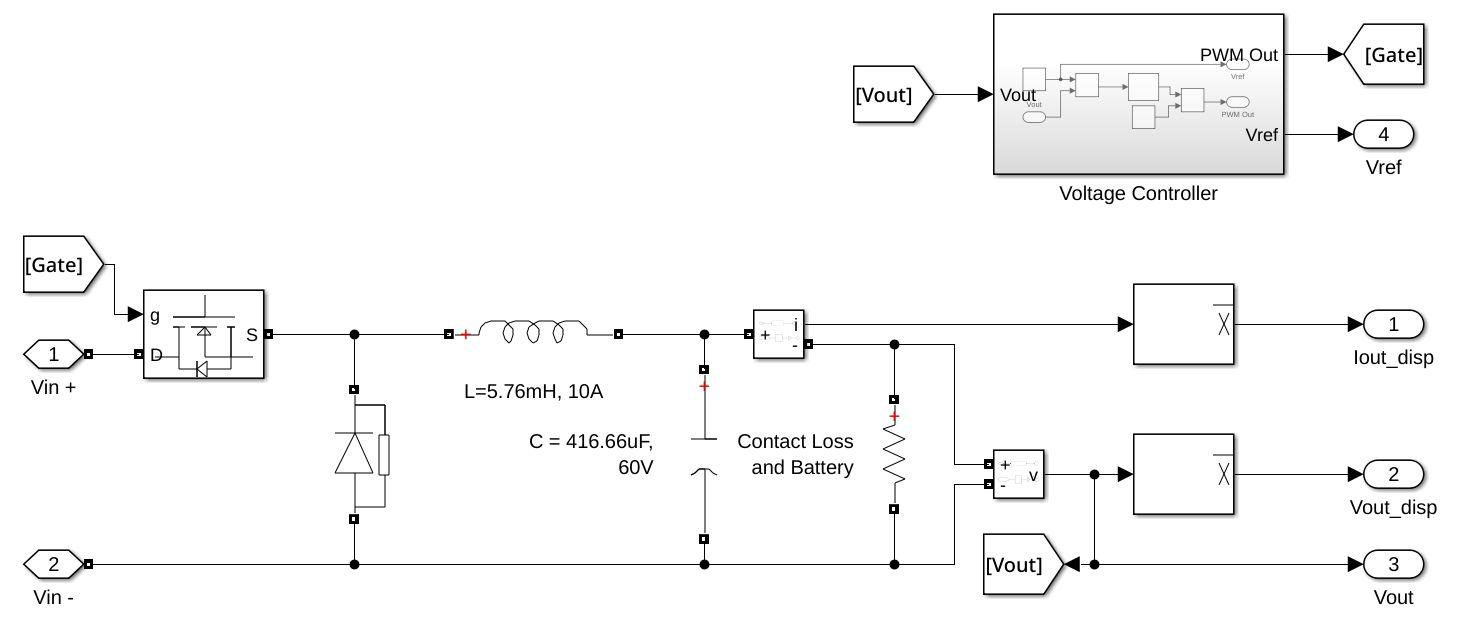
\includegraphics[width=0.8\textwidth]{img/Buck_Circuit.jpg}
    \caption{Buck Converter}
\end{figure}

A Buck Converter is a type of DC-DC converter that steps down a higher input voltage (\(V_{\text{in}}\)) to a lower output voltage (\(V_{\text{out}}\)) by switching a transistor (MOSFET) on and off at high frequency (10kHz). This circuit is controlled by a \textbf{PWM (Pulse Width Modulation)} signal that adjusts the output voltage based on the desired reference voltage (\(V_{\text{ref}}\)).

\section*{Components and Operation}

\subsection*{1. Input Voltage (\(V_{\text{in}}\))}
The input voltage source (\(V_{\text{in}}\)) provides the initial DC power to the Buck converter. This voltage is typically higher than the required output voltage.

\subsection*{2. Switching MOSFET}
The MOSFET acts as a high-speed electronic switch controlled by a \textbf{PWM signal}. The switching operation determines the duty cycle of the output, which in turn controls the average output voltage. When the MOSFET is turned on (closed), current flows through the inductor to the load. When it’s off (open), the inductor maintains the current flow by releasing its stored energy.

In this Buck Converter, the MOSFET is switched at a frequency of 10 kHz. The switching frequency is chosen based on a balance between efficiency, component size, and heat dissipation. Here’s why 10 kHz is a suitable choice:

\begin{itemize}
    \item \textbf{Efficiency vs. Switching Losses:} Higher switching frequencies improve the output voltage ripple and dynamic response but also increase switching losses in the MOSFET. At 10 kHz, switching losses are kept relatively low, helping to maintain high overall efficiency without excessive heat generation in the MOSFET.
    \item \textbf{Component Sizing:} Inductors and capacitors can be smaller at higher switching frequencies because the ripple current and voltage decrease as frequency increases. However, very high frequencies (e.g., above 100 kHz) require expensive high-speed MOSFETs and may lead to electromagnetic interference (EMI) issues. A frequency of 10 kHz allows for a reasonable component size while balancing performance and cost.
\end{itemize}

\subsection*{3. Diode}
The diode provides a path for the inductor current when the MOSFET is off, preventing reverse current. This configuration helps maintain a steady current flow to the load.

\subsection*{4. Inductor (\(L = 5.76\text{mH}, 10A\))}
The inductor stores energy when the MOSFET is ON and releases it when the MOSFET is OFF. It smooths the current flow to reduce ripple, making the output current more stable. The inductance value here is 5.76 mH, and allows it to handle a maximum current of 10 A.

\subsubsection*{Inductance Value Selection in the Buck Converter}
The inductance value (\(L\)) in a Buck Converter is chosen to limit the ripple current (\(\Delta I_L\)) through the inductor. Controlling this current ripple helps improve efficiency, reduce stress on components, and maintain a stable output current. In this converter, the inductance value is calculated to keep \(\Delta I_L\) within 10\% of the output current.

\[
L = \frac{V_{\text{out}} \cdot (1-D)}{f_s \cdot \Delta I_L}
\]

where:
\begin{itemize}
    \item \(V_{\text{out}}\) is the output voltage,
    \item \(D\) is the duty cycle,
    \item \(f_s\) is the switching frequency (10 kHz in this case),
    \item \(\Delta I_L\) is the peak-to-peak ripple current through the inductor.
\end{itemize}

Given the following values:
\begin{itemize}
    \item \(V_{\text{out}} = 48V\),
    \item \(f_s = 10 \text{kHz}\),
    \item \(\Delta I_L = 0.5A\),
\end{itemize}

The inductance is calculated to be \(5.76 \text{mH}\), and the current rating of 10A is chosen to handle transients.

\subsection*{5. Capacitor (\(C = 416.66\mu F, 60V\))}
The capacitor at the output helps to further smooth the output voltage by reducing ripple. This filter capacitor is crucial for maintaining a steady DC output. Its capacitance is 416.66 µF, rated for 60 V.

\subsubsection*{Capacitance Value Selection in the Buck Converter}
The capacitance value (\(C\)) in a Buck Converter is chosen to limit the ripple voltage (\(\Delta V_{\text{out}}\)) across the output capacitor. Controlling this voltage ripple helps maintain a stable output voltage and reduce noise, ensuring reliable operation of the load. In this converter, the capacitance value is calculated to keep \(\Delta V_{\text{out}}\) within an acceptable range, typically within 1-2\% of the output voltage.

\[
C = \frac{I_{\text{out}}}{f_s \cdot \Delta V_{\text{out}}}
\]
\newpage
where:
\begin{itemize}
    \item \(I_{\text{out}}\) is the output current,
    \item \(D\) is the duty cycle,
    \item \(f_s\) is the switching frequency (10 kHz in this case),
    \item \(\Delta V_{\text{out}}\) is the peak-to-peak ripple voltage at the output.
\end{itemize}

After substituting the values:
\begin{itemize}
    \item \(V_{\text{out}} = 48V\),
    \item \(I_{\text{out}} = 5A\),
    \item \(f_s = 10 \text{kHz}\),
    \item \(\Delta V_{\text{out}} = 0.48V\),
\end{itemize}

The capacitance comes out to be 416.66µF.

\subsection*{6. Contact Loss and Battery}
This block represents the connection to the load, including any contact resistance or battery characteristics. Contact loss simulates any additional resistance or drop caused by imperfect contacts, which may affect the efficiency of power transfer.

\subsection*{7. Voltage Controller}
The \textbf{Voltage Controller} block compares the output voltage (\(V_{\text{out}}\)) with the reference voltage (\(V_{\text{ref}}\)) and adjusts the PWM signal sent to the MOSFET gate to regulate the output. This feedback loop helps maintain a steady output voltage regardless of input or load variations.

\subsection*{8. Output Voltage (\(V_{\text{out}}\))}
The output voltage (\(V_{\text{out}}\)) is the regulated, stepped-down voltage delivered to the load. It’s continuously monitored by the Voltage Controller to ensure it remains close to \(V_{\text{ref}}\).

\section*{PI Controller}
\subsection*{Overview}
A \textbf{PI (Proportional-Integral)} controller is a type of feedback controller used to maintain a system’s output at a desired level by adjusting the input control signal. It is commonly used in control systems to eliminate steady-state error and provide a stable response.

\subsection*{Components and Operation}

\begin{itemize}
    \item \textbf{Error Signal (e(t))} \\
    The error signal \( e(t) \) is the difference between the reference value (desired output) and the actual output of the system. This error drives the PI controller, determining how much correction is needed.

    \item \textbf{Proportional Term (P)} \\
    The proportional term provides an output that is directly proportional to the error signal. This term is responsible for reducing the magnitude of the error, improving the response speed:

    \[
    P_{\text{out}} = K_p \times e(t)
    \]

    Where \( K_p \) is the proportional gain, which dictates how aggressively the controller reacts to the error.

    \item \textbf{Integral Term (I)} \\
    The integral term accumulates the error over time, addressing any steady-state error that the proportional term alone cannot eliminate. This helps the system reach the exact target over time:

    \[
    I_{\text{out}} = K_i \int e(t) \, dt
    \]

    Where \( K_i \) is the integral gain, which controls the response to accumulated errors.

    \item \textbf{Combined PI Output} \\
    The overall output of the PI controller is the sum of the proportional and integral terms, providing a balance between fast response and steady-state accuracy:

    \[
    \text{PI}_{\text{out}} = P_{\text{out}} + I_{\text{out}} = K_p \cdot e(t) + K_i \int e(t) \, dt
    \]

    This combined output is used to adjust the system’s input, aiming to minimize the error over time.

    \item \textbf{Effect of Tuning Parameters} \\
    The gains \( K_p \) and \( K_i \) need to be carefully tuned to achieve a desirable system response:
    \begin{itemize}
        \item \textbf{Increasing \( K_p \)} improves response speed but may lead to overshoot or oscillation.
        \item \textbf{Increasing \( K_i \)} helps eliminate steady-state error but may cause slow settling or instability if set too high.
    \end{itemize}
    \item \textbf{Tuned PI Values} \\
    After tuning the PI controller, the \( K_p \) was found out to be 0.001 and \( K_i \) was found out to be 0.07.

\end{itemize}
\section*{Procedure}

\begin{enumerate}
    \item \textbf{Initial Setup with Resistive Load:} A 322$\Omega$ resistor was initially used as a load to simulate a 1A current supply from the FWR.
    \item \textbf{Resistive Load Adjustment:} The resistor value was later changed to 322$\Omega / 2 = 161\Omega$ to simulate a higher current demand of 2A.
    \item \textbf{Replacement with Buck Converter:} After testing with resistive loads, a buck converter was connected in place of the resistive load. The buck converter helps step down the voltage while maintaining a stable current of 48V and 5A for the e-bike battery charging application.
    \begin{itemize}
        \item The transition from resistive load to buck converter was made to improve efficiency and provide regulated DC output suitable for e-bike charging.
        \item The system was tested under different load conditions, and the performance was validated with the buck converter to ensure it meets the power requirements.
    \end{itemize}
\end{enumerate}

\section*{Power Factor Correction (PFC)}
The PFC circuit ensures a sinusoidal, in-phase current draw from the grid, improving the power factor and reducing harmonic distortion. This enhancement improves the overall efficiency of the charging system and ensures compliance with grid standards for power quality.

\subsection*{Boost Converter}
\begin{itemize}
    \item Positioned after the Full-Wave Rectifier (FWR) and before the Buck Converter in the circuit.
    \item Regulates the input current to match a sinusoidal reference, correcting the power factor by shaping the current waveform to follow the grid voltage.
\end{itemize}

\subsection*{Sine Reference}
\begin{itemize}
    \item A sine reference sets the desired current waveform to ensure the grid current is sinusoidal. The PFC circuit uses two PI controllers to adjust the duty cycle of the boost converter in response to this reference.
    \item The outer PI controller regulates the boost converter’s output voltage, adjusting the reference current for the inner loop.
    \item The inner PI controller controls the duty cycle of the boost converter, ensuring that the input current follows the sinusoidal reference waveform and stays in phase with the grid voltage.
\end{itemize}
This synchronization of current and voltage results in a sinusoidal current draw from the grid, which improves the overall power factor.
\begin{figure}[h]
    \centering
    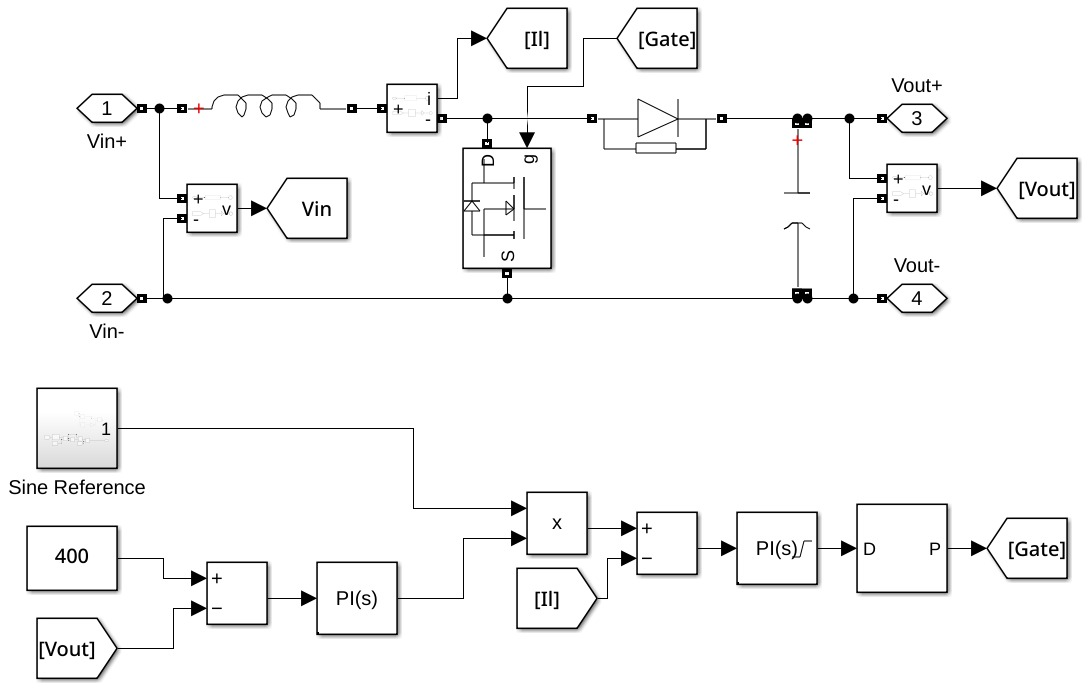
\includegraphics[width=0.8\textwidth]{img/pfc_circuit.jpg}
    \caption{PFC Circuit}
\end{figure}


\subsection*{PI Controllers}
\begin{enumerate}
    \item \textbf{Outer PI Controller (Voltage Loop):}
    \begin{itemize}
        \item Controls the output voltage of the boost converter, keeping it stable by adjusting the reference current fed to the inner controller.
        \item  After tuning this PI controller, the \( K_p \) was found out to be 0.25 and \( K_i \) was found out to be 35.

    \end{itemize}
    \item \textbf{Inner PI Controller (Current Loop):}
    \begin{itemize}
        \item Regulates the input current, ensuring it follows a sinusoidal reference waveform that is in phase with the grid voltage. This results in a high power factor and efficient power transfer.
        \item  After tuning this PI controller, the \( K_p \) was found out to be 2000 and \( K_i \) was found out to be 0.25.

    \end{itemize}
\end{enumerate}

\subsection*{Circuit Benefits}
\begin{itemize}
    \item \textbf{Power Factor Correction:} Aligns the input current with the grid voltage, reducing reactive power and enhancing efficiency.
    \item \textbf{Harmonic Reduction:} The sinusoidal current draw minimizes harmonic distortion, ensuring cleaner power from the grid.
    \item \textbf{Increased Efficiency:} The PFC improves the overall efficiency of the system by optimizing the energy drawn from the grid, making the charging process more effective and sustainable.
\end{itemize}
\begin{figure}[h]
    \centering
    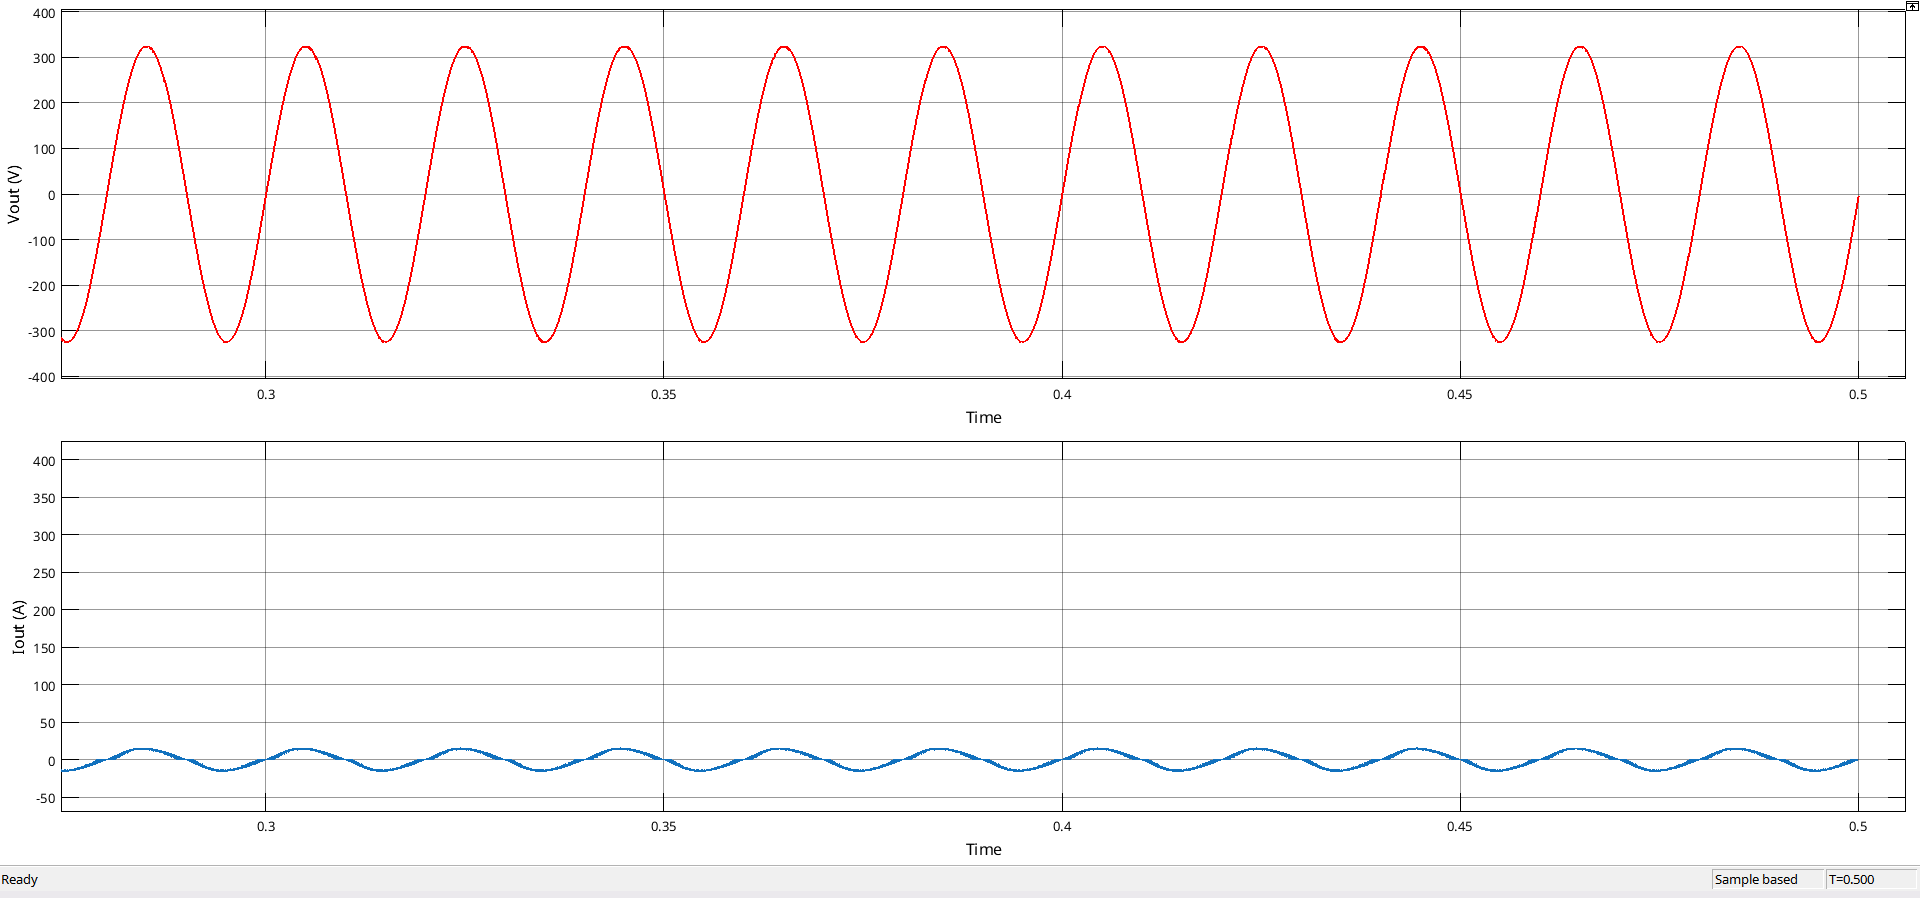
\includegraphics[width=0.6\textwidth]{img/InputVnI.png}
    \caption{Grid Input Voltage and Current with PFC}
\end{figure}


\newpage
\section*{Results}

The Full Bridge Rectifier's output with a 1A load yielded a ripple of 3.01V, which meant that if the load consumes less than 1A, it will be within the 1\% limit.

\begin{figure}[h]
    \centering
    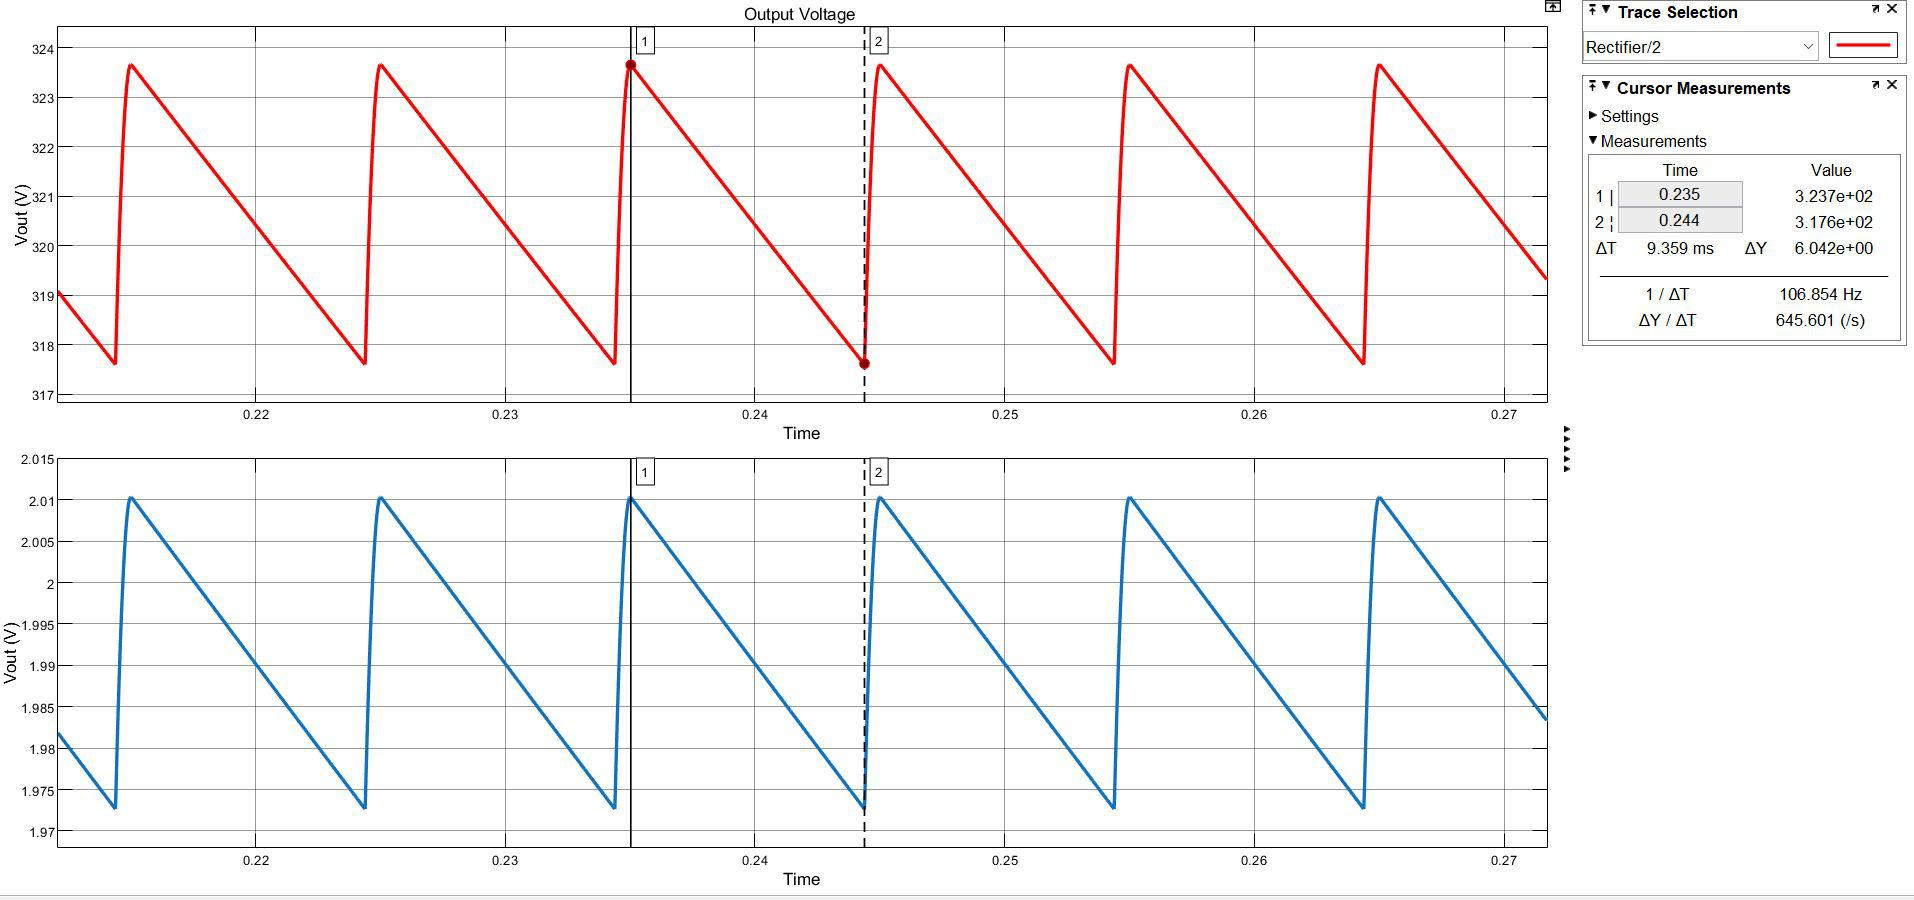
\includegraphics[width=0.8\textwidth]{img/2A_n.jpg}
    \caption{2A Load Ripple}

    \centering
    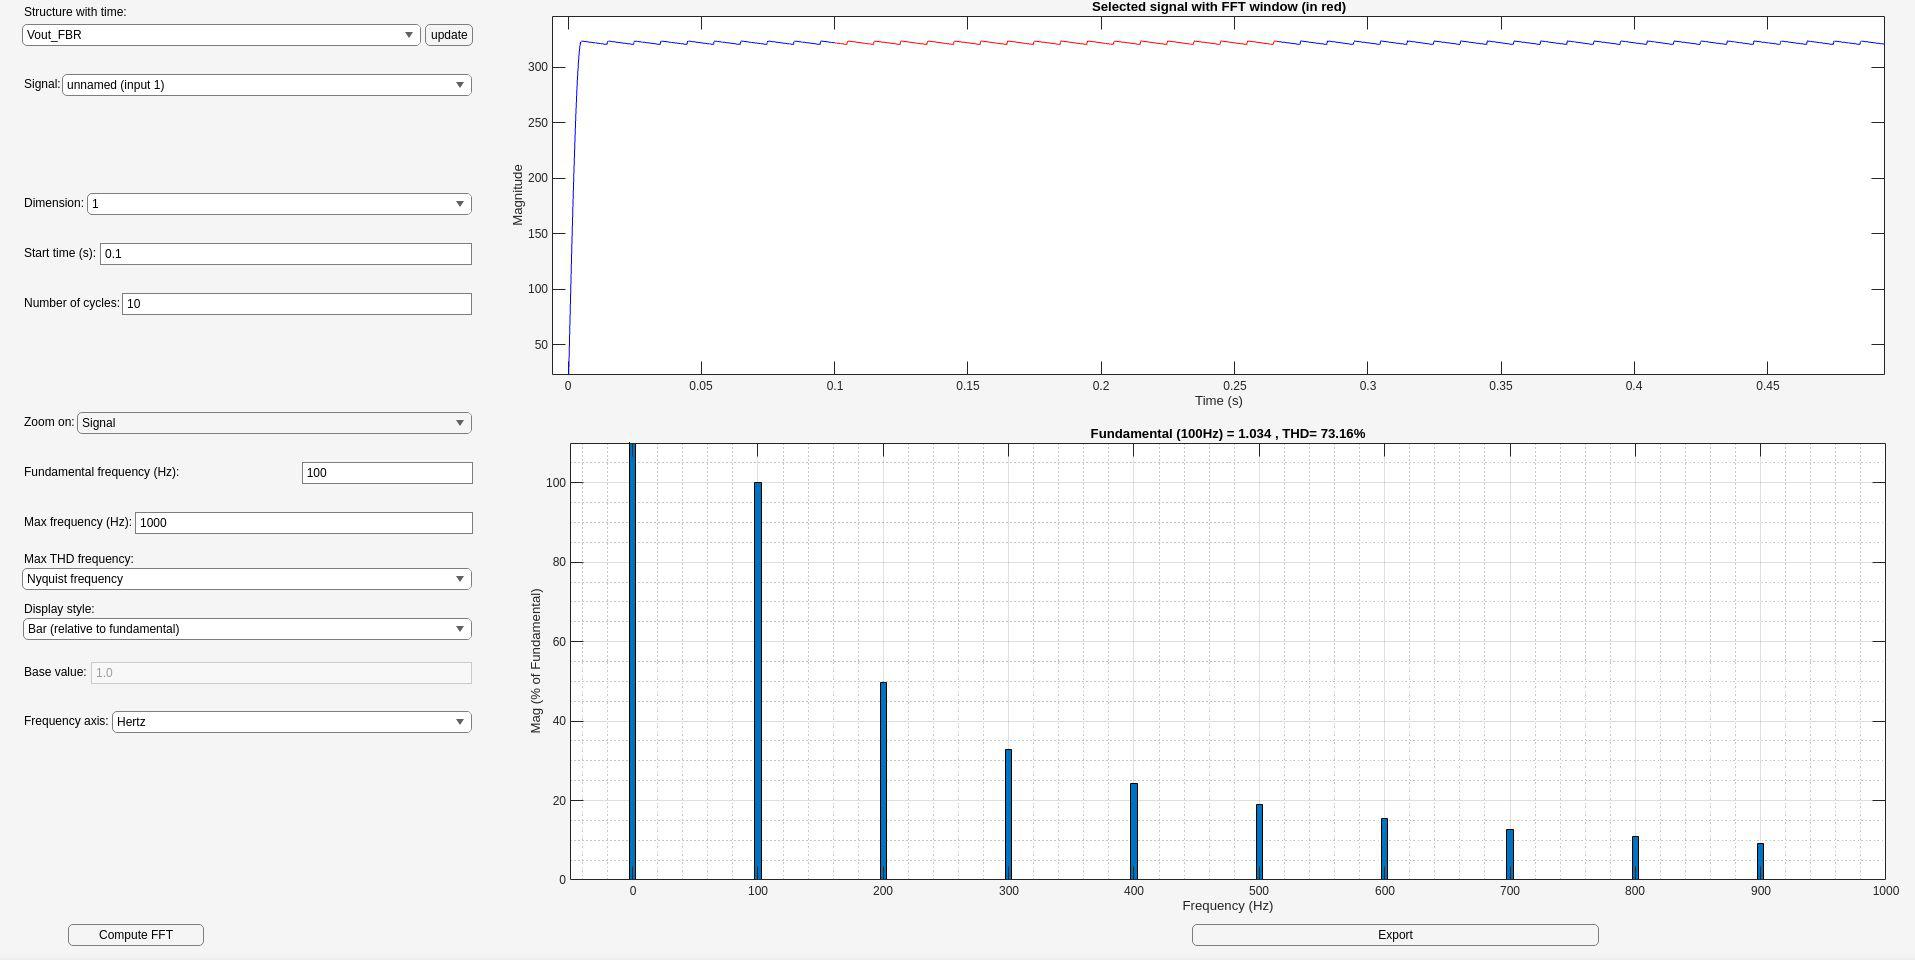
\includegraphics[width=0.7\textwidth]{img/FBR_1A.jpg}
    \caption{Full Bridge Rectifier Output with 1A Load (TDR)}
\end{figure}
\newpage
The Full Bridge Rectifier's output with a 2A load yielded a ripple of 3.395V, while the expected ripple was supposed to be 7.02V.

\begin{figure}[h]
    \centering
    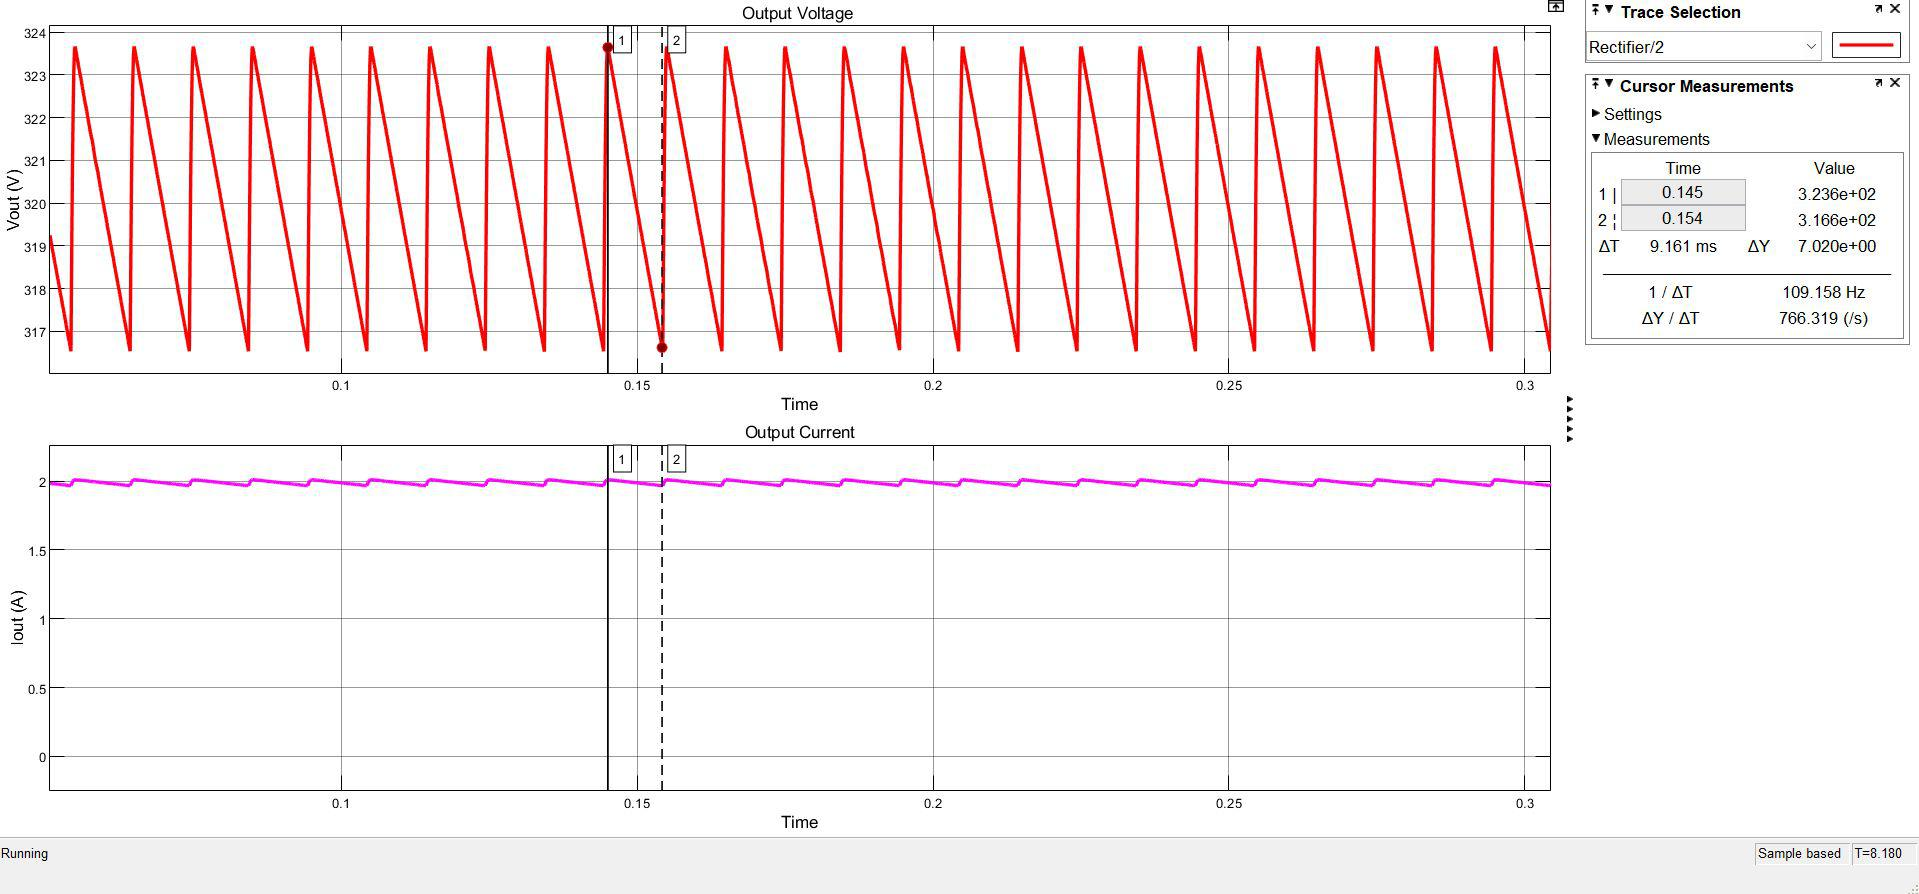
\includegraphics[width=0.8\textwidth]{img/2A.jpg}
    \caption{2A Load Ripple}

    \centering
    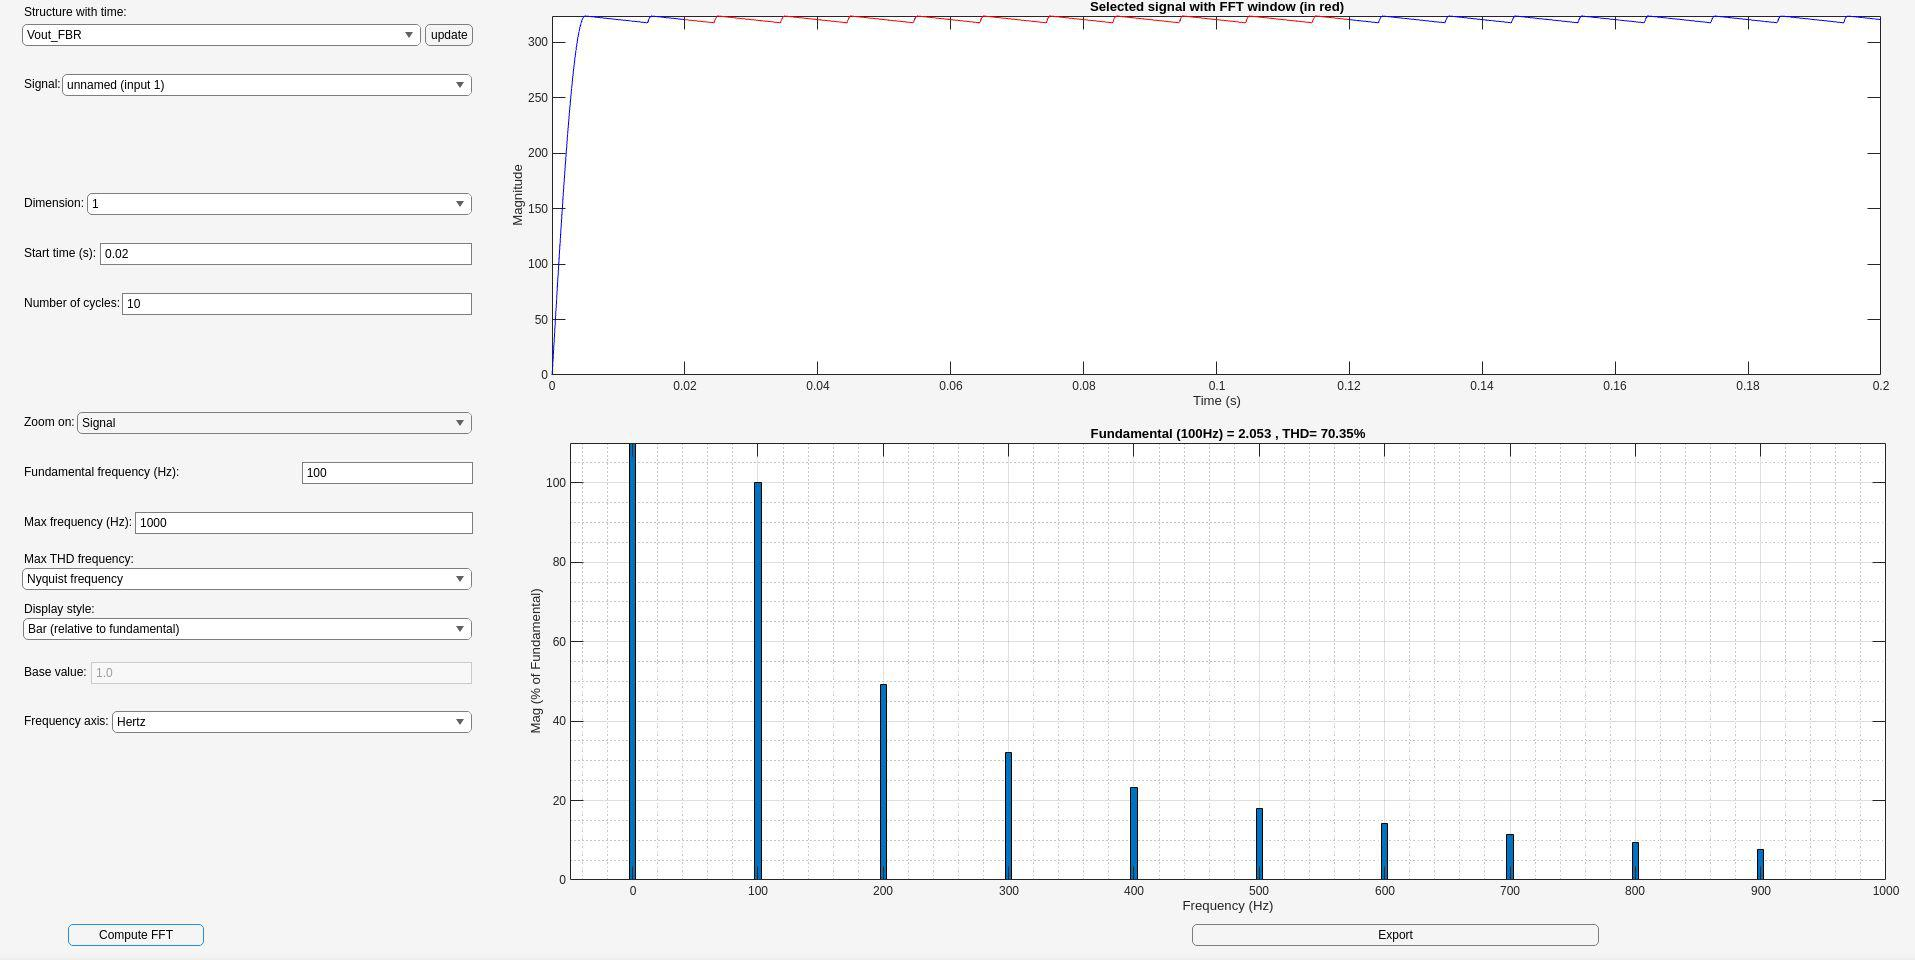
\includegraphics[width=0.8\textwidth]{img/FBR_2A.jpg}
    \caption{Full Bridge Rectifier Output with 2A Load (TDR)}
\end{figure}
\newpage

Since the load resistance is decreased, the capacitor discharges very quickly between the pulsating rectified voltage peaks. This fast discharging causes a bigger percentage drop in the output voltage during the intervals between the peaks of the rectified voltage, which increases ripple voltage.\\

When the capacitance values were increased, the ripples were reduced to below 1\%.

\begin{figure}[h]
    \centering
    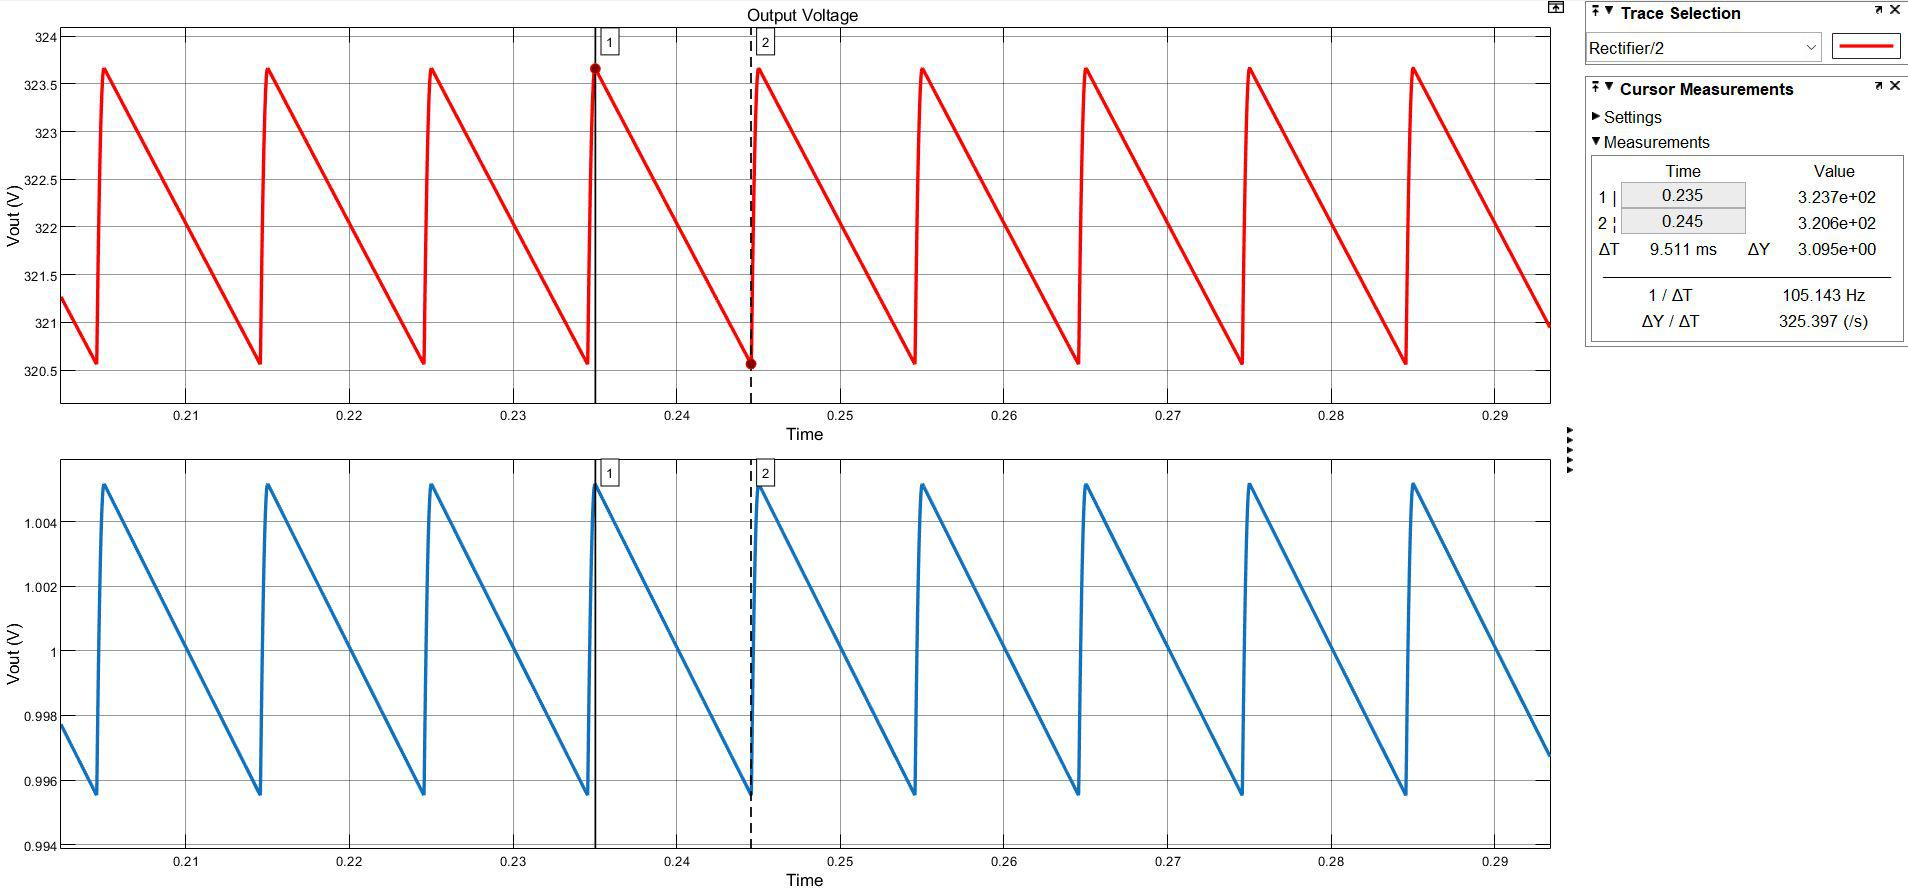
\includegraphics[width=0.8\textwidth]{img/1A.jpg}
    \caption{Reduced Ripple with Increased Capacitance (1A Load)}

    \centering
    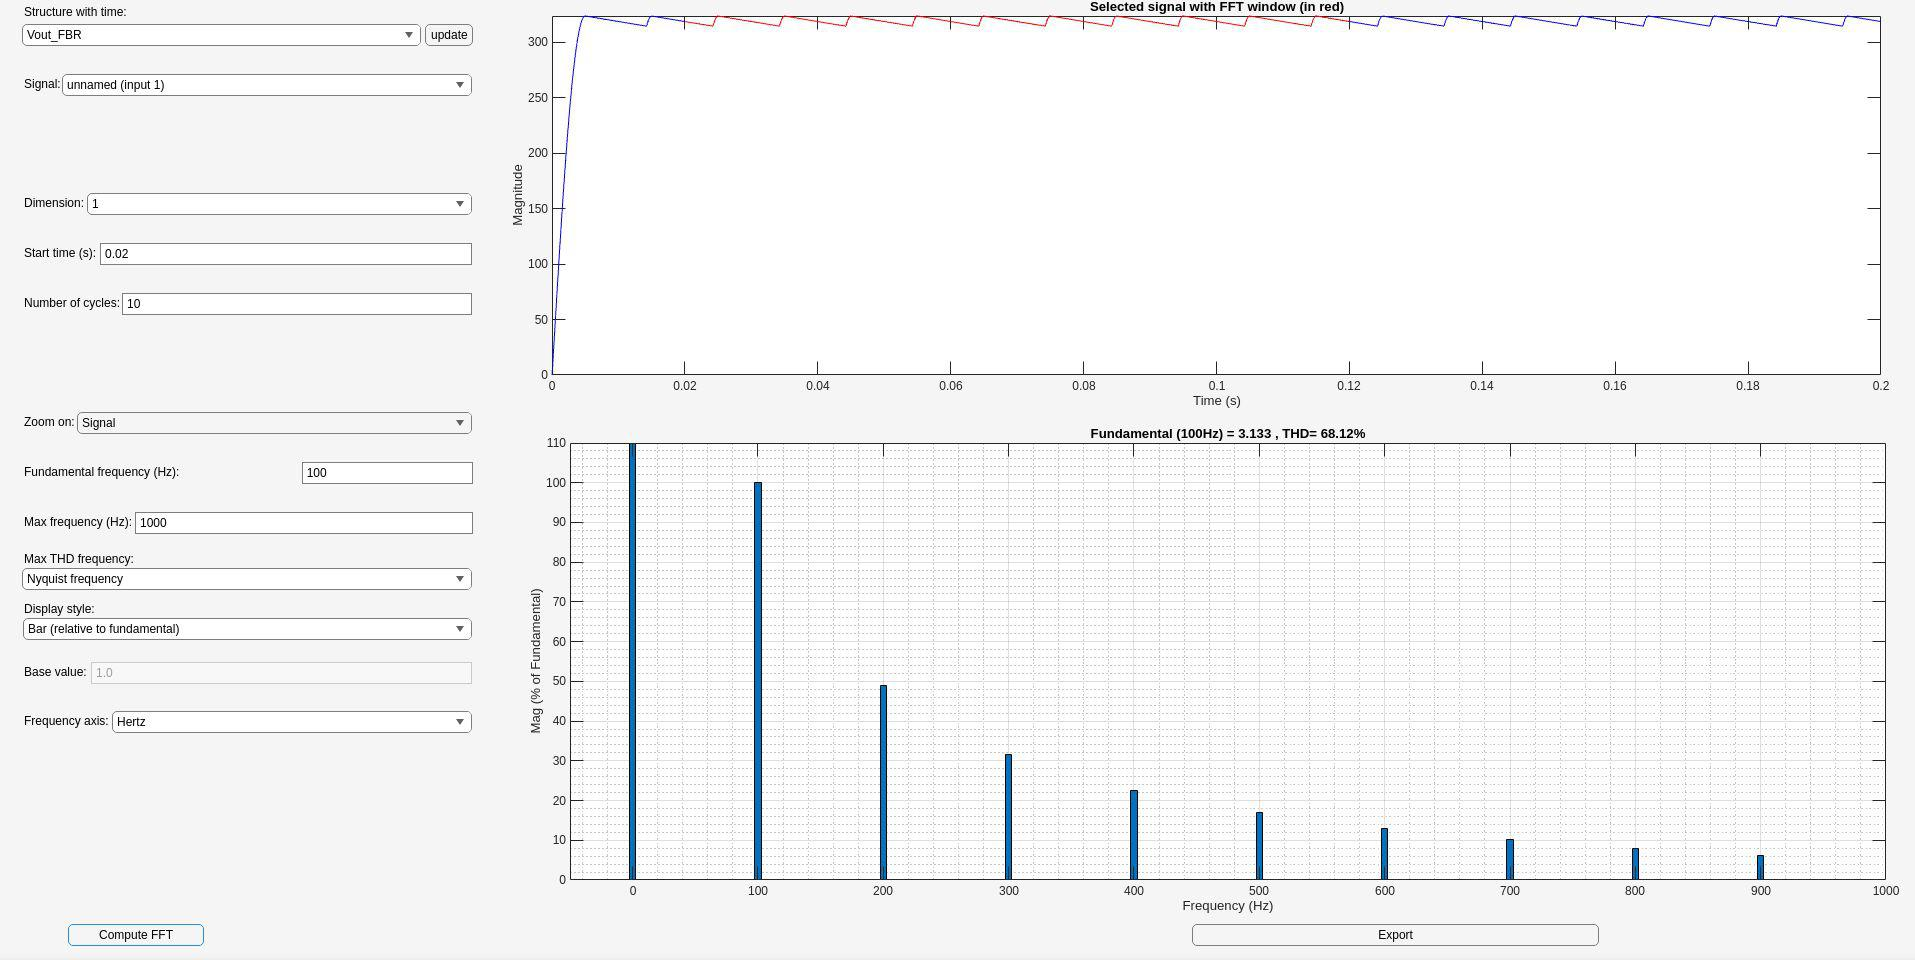
\includegraphics[width=0.8\textwidth]{img/FBR_1A_n.jpg}
    \caption{Full Bridge Rectifier Output with Increased Capacitance (TDR)}
\end{figure}
\newpage

When the load resistor was removed and attached to the buck converter, the FBR's output voltage ripple was around 2.43V, which is below the 1\% limit.
\begin{figure}[h]
    \centering
    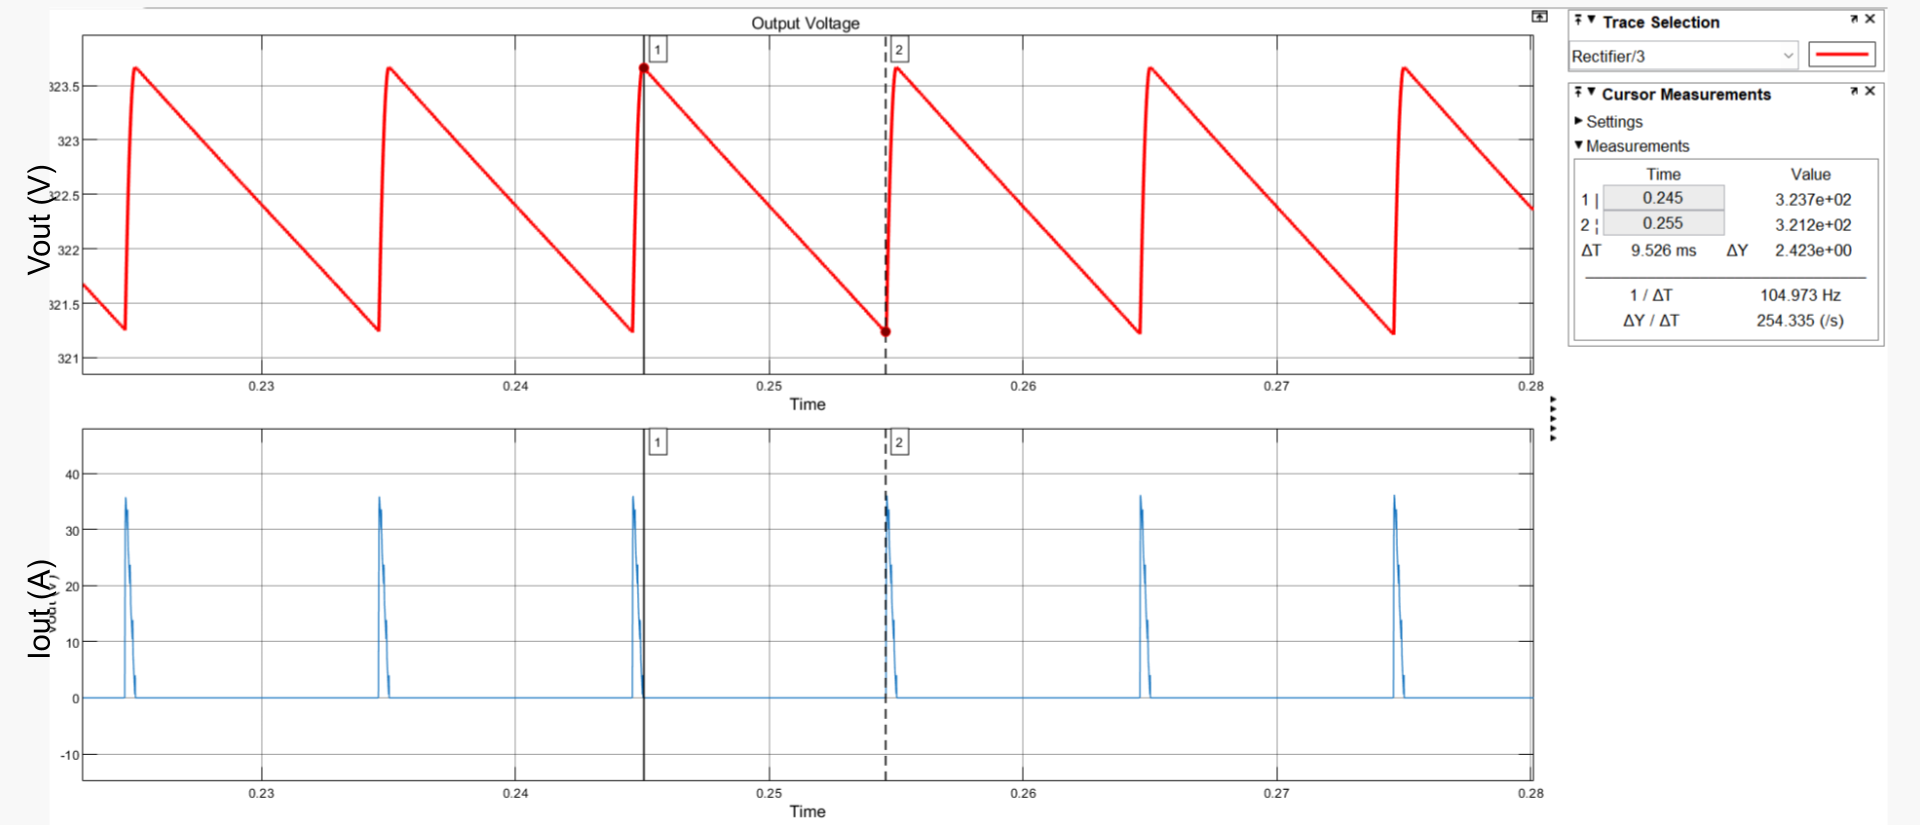
\includegraphics[width=0.8\textwidth]{img/FBR_Buck_graph.png}
    \caption{FBR output with Buck Load}
    \centering
    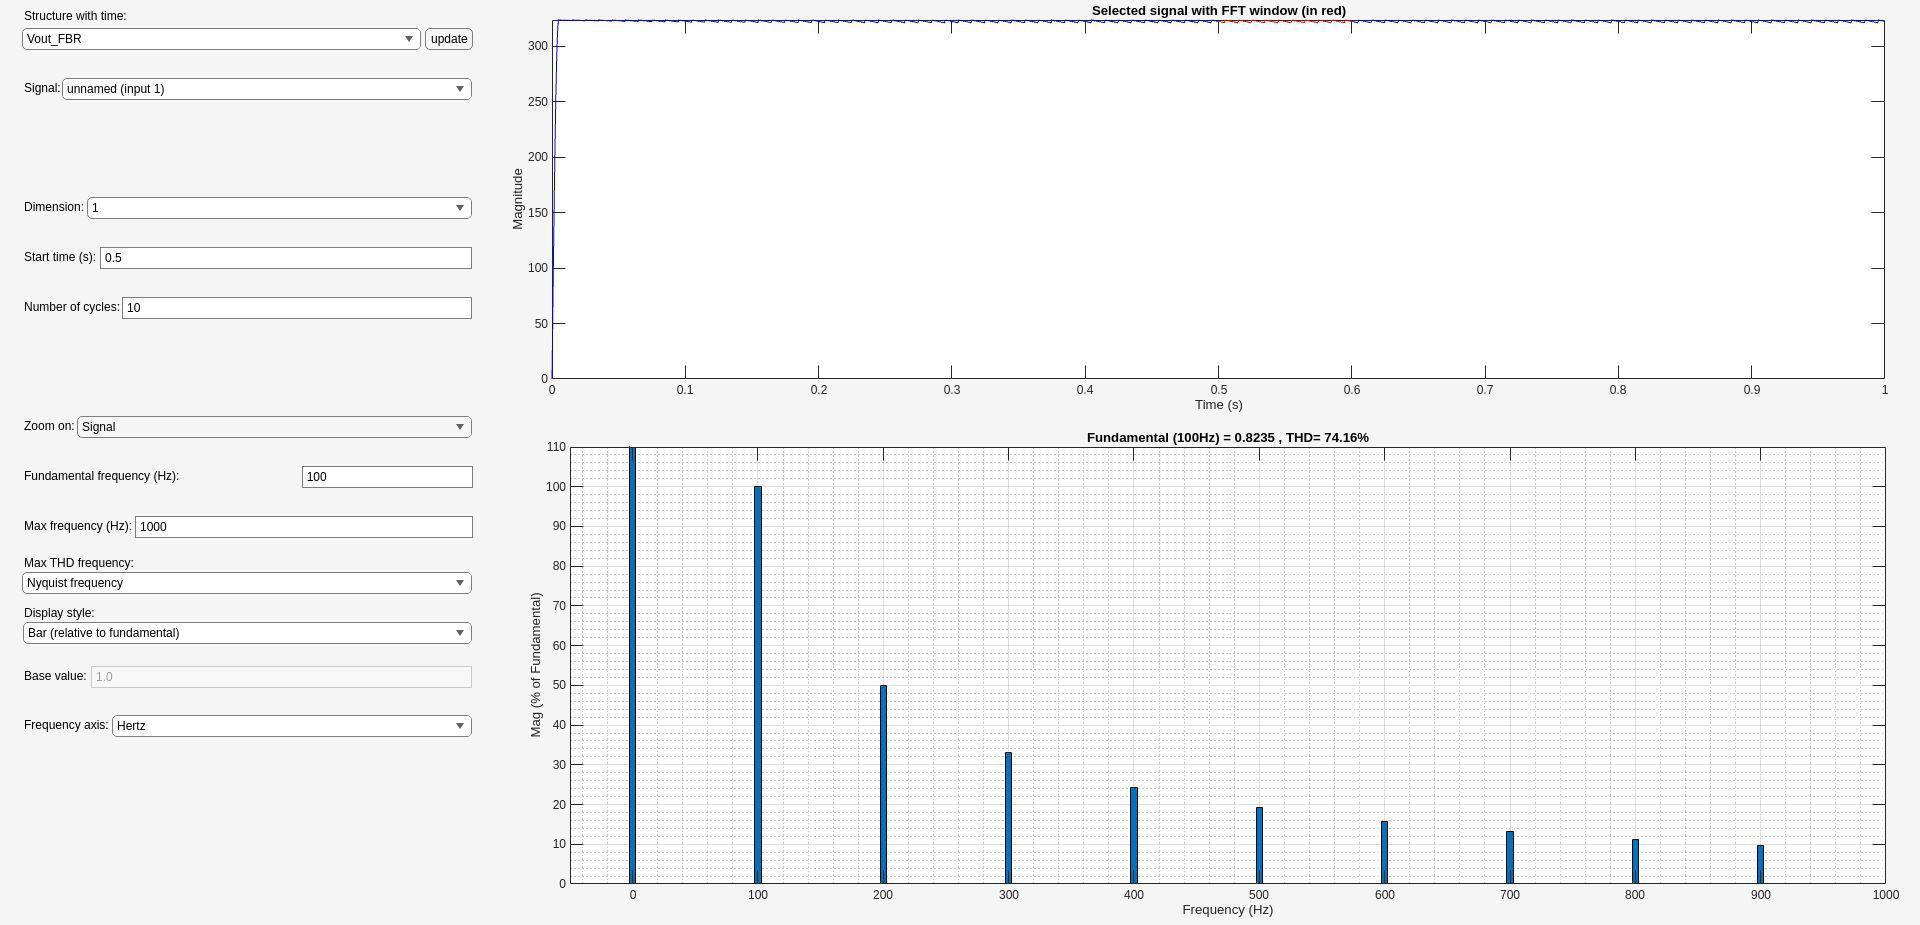
\includegraphics[width=0.8\textwidth]{img/FBR_Buck.jpg}
    \caption{Full Bridge Rectifier Output with Buck Load (TDR)}
\end{figure}

\newpage

The buck converter's output voltage and current was observed to be within the limit of 1\%.

\begin{figure}[h]
    \centering
    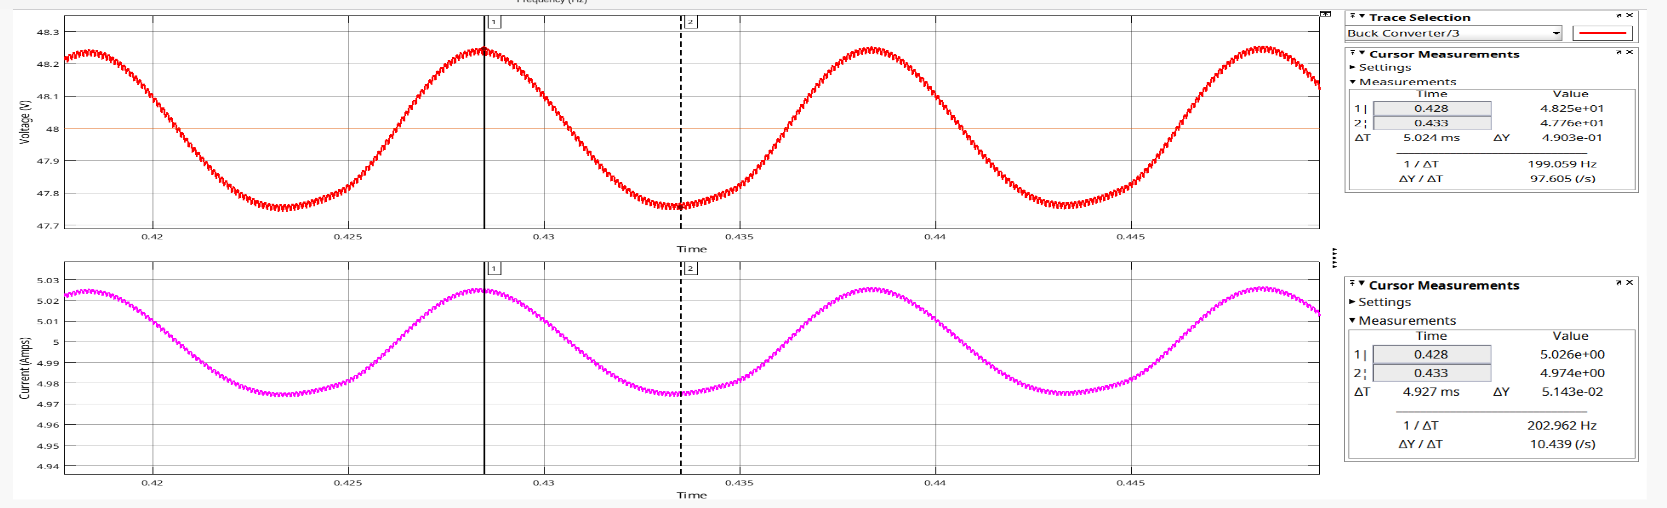
\includegraphics[width=0.6\textwidth]{img/Buck_VnI.png}
    \caption{Buck Converter Output}

    \centering
    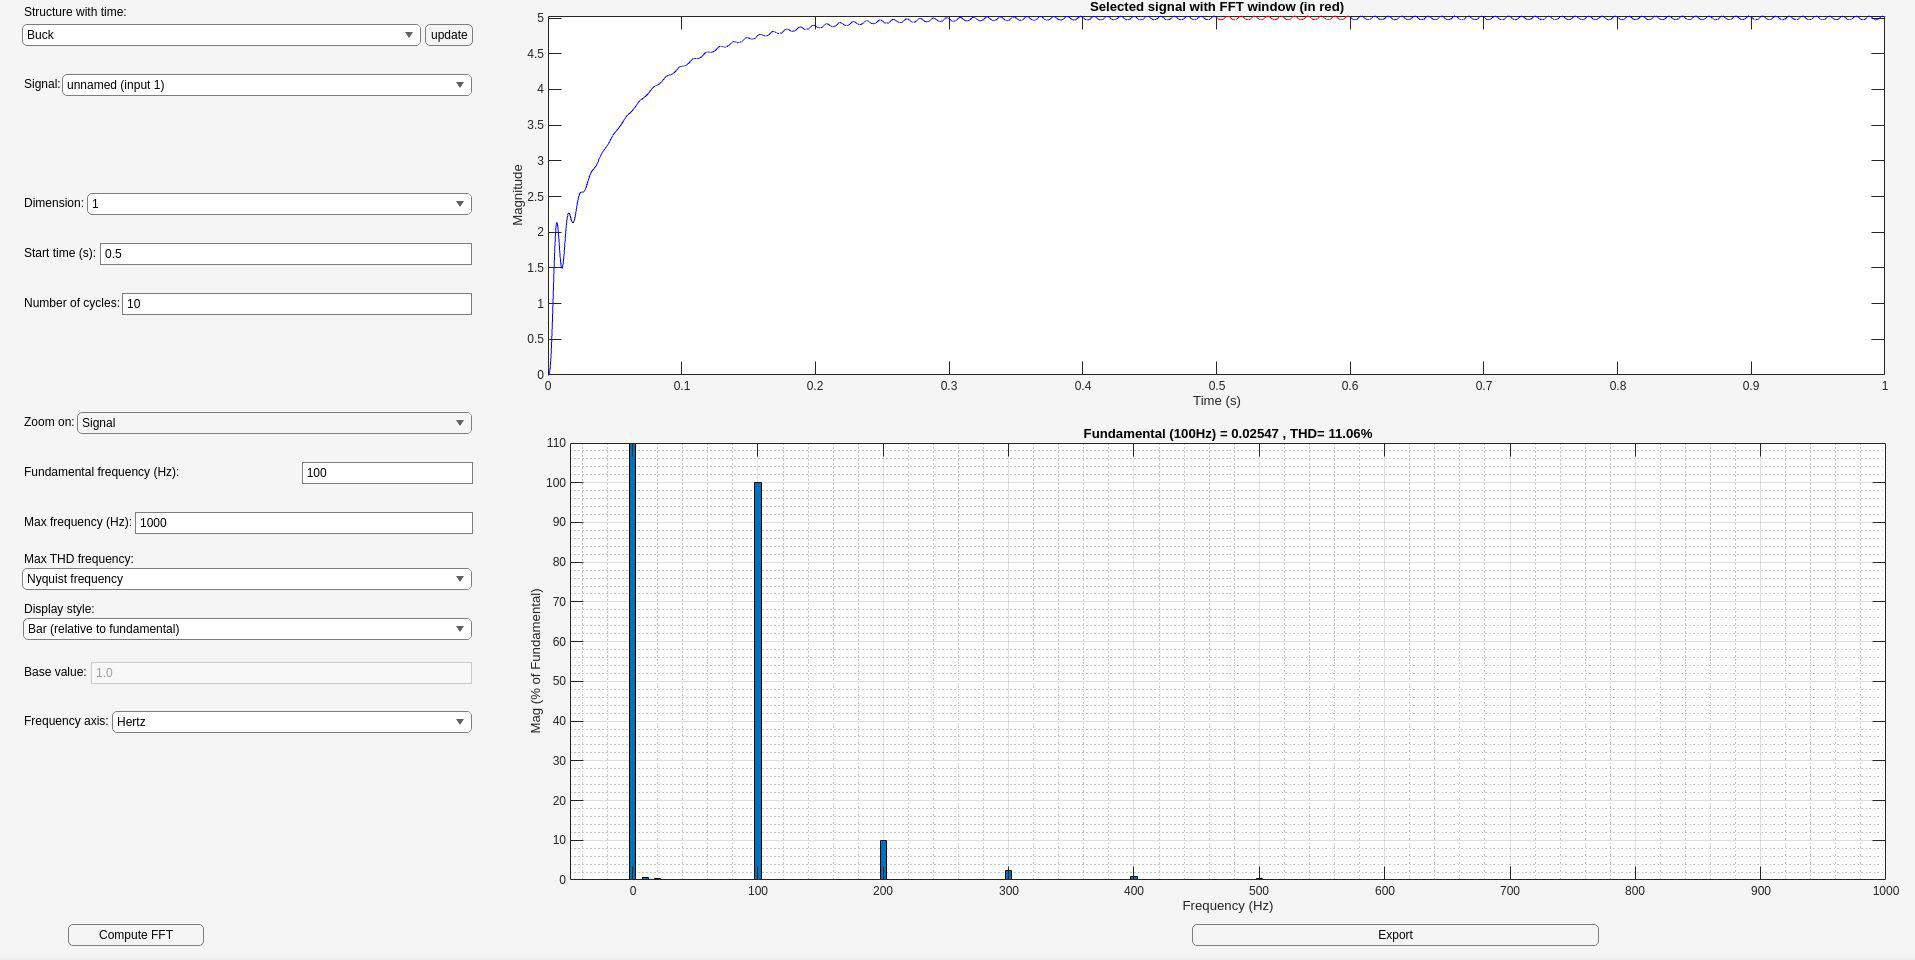
\includegraphics[width=0.6\textwidth]{img/Buck_Iout.jpg}
    \caption{Buck Converter Output Current (TDR)}

    \centering
    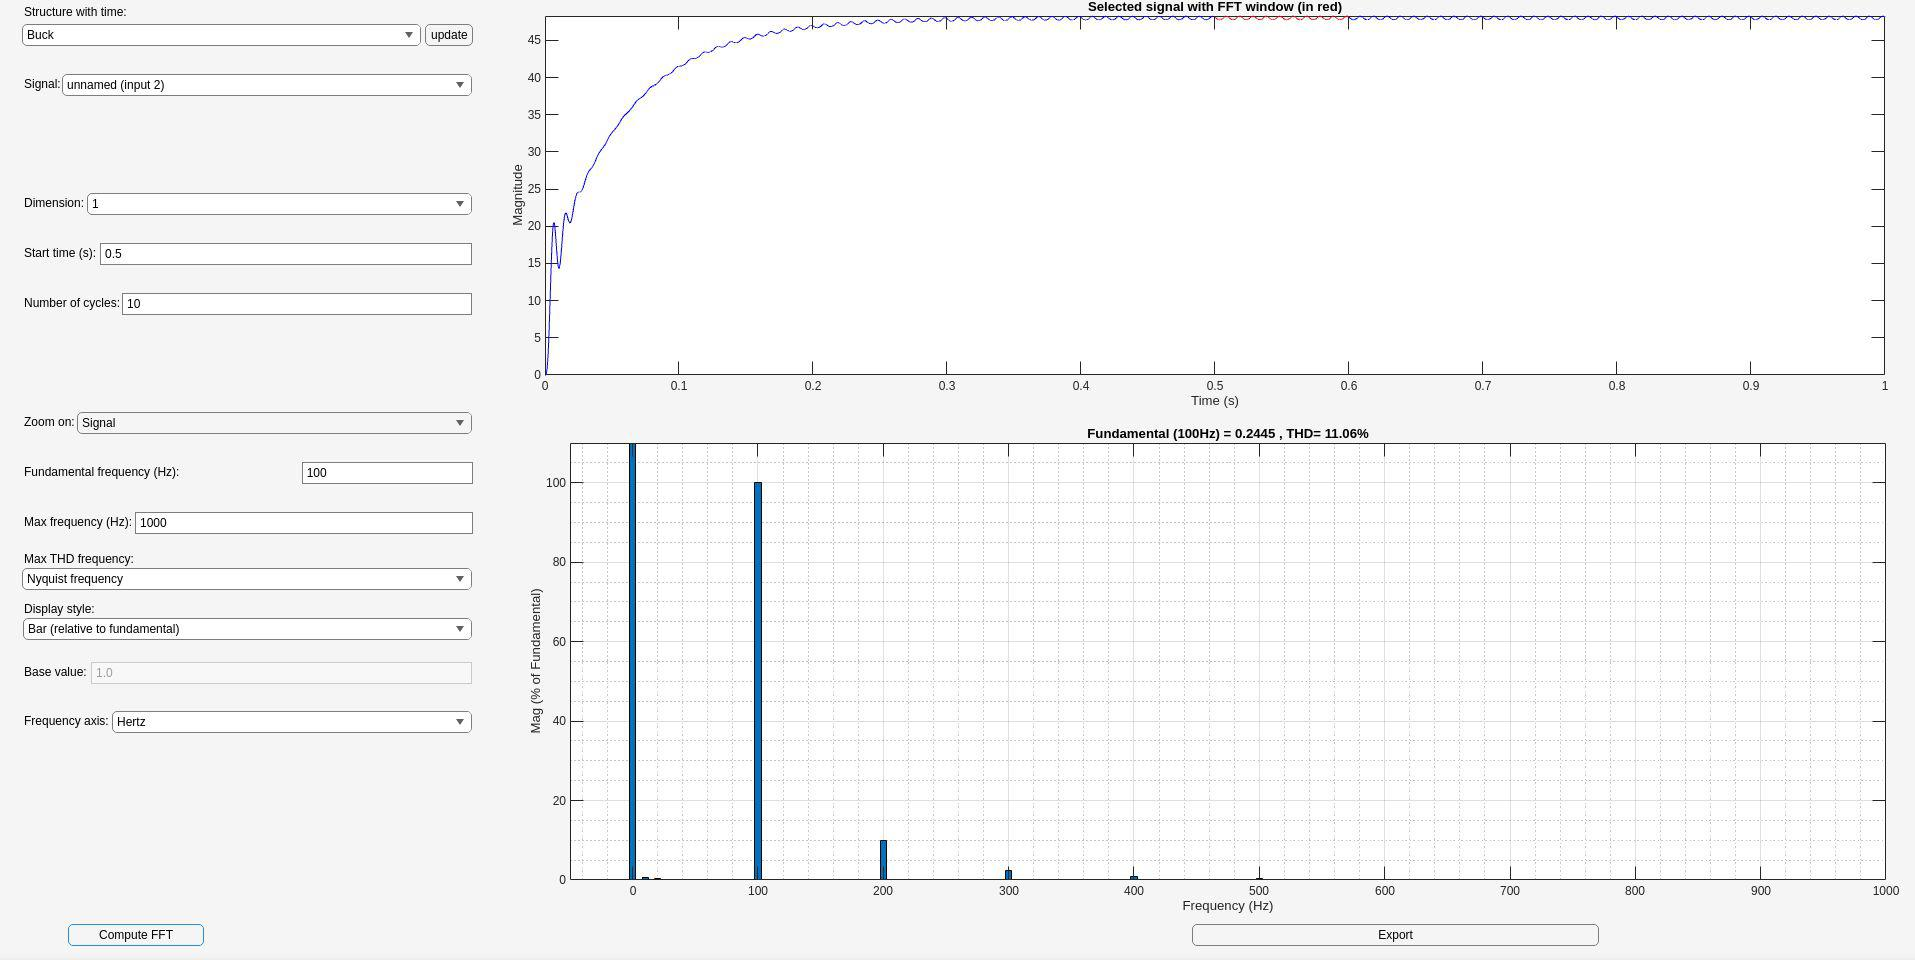
\includegraphics[width=0.6\textwidth]{img/Buck_Vout.jpg}
    \caption{Buck Converter Output Voltage (TDR)}
\end{figure}

\newpage

\section*{Conclusion}
In this project, we successfully integrated a FWR with a buck converter to create a reliable and efficient 48V, 5A e-bike charger. By using a PID-controlled buck converter, the system achieves a stable output suitable for e-bike battery charging, while minimizing ripple at the rectifier's output. The constant current draw from the rectifier ensures reduced fluctuations and ripple, making the charger both efficient and well-suited for high-demand applications like e-bikes.\\
The power consumed from the grid by this onboard charger was 257.4\,\text{W}, and the power output was 239.5\,\text{W}, which gives it an efficiency of 93.04\%.\\

\[
\text{Efficiency} = \frac{\text{Power Output}}{\text{Power Input}} \times 100\% = \frac{239.5\,\text{W}}{257.4\,\text{W}} \times 100\% = 93.04\%
\]

When the PFC circuit was added, the buck converter’s output voltage’s TDH dropped to 2.66\%, which showed how important PFC is in a charger circuit.
\begin{figure}[h]
    \centering
    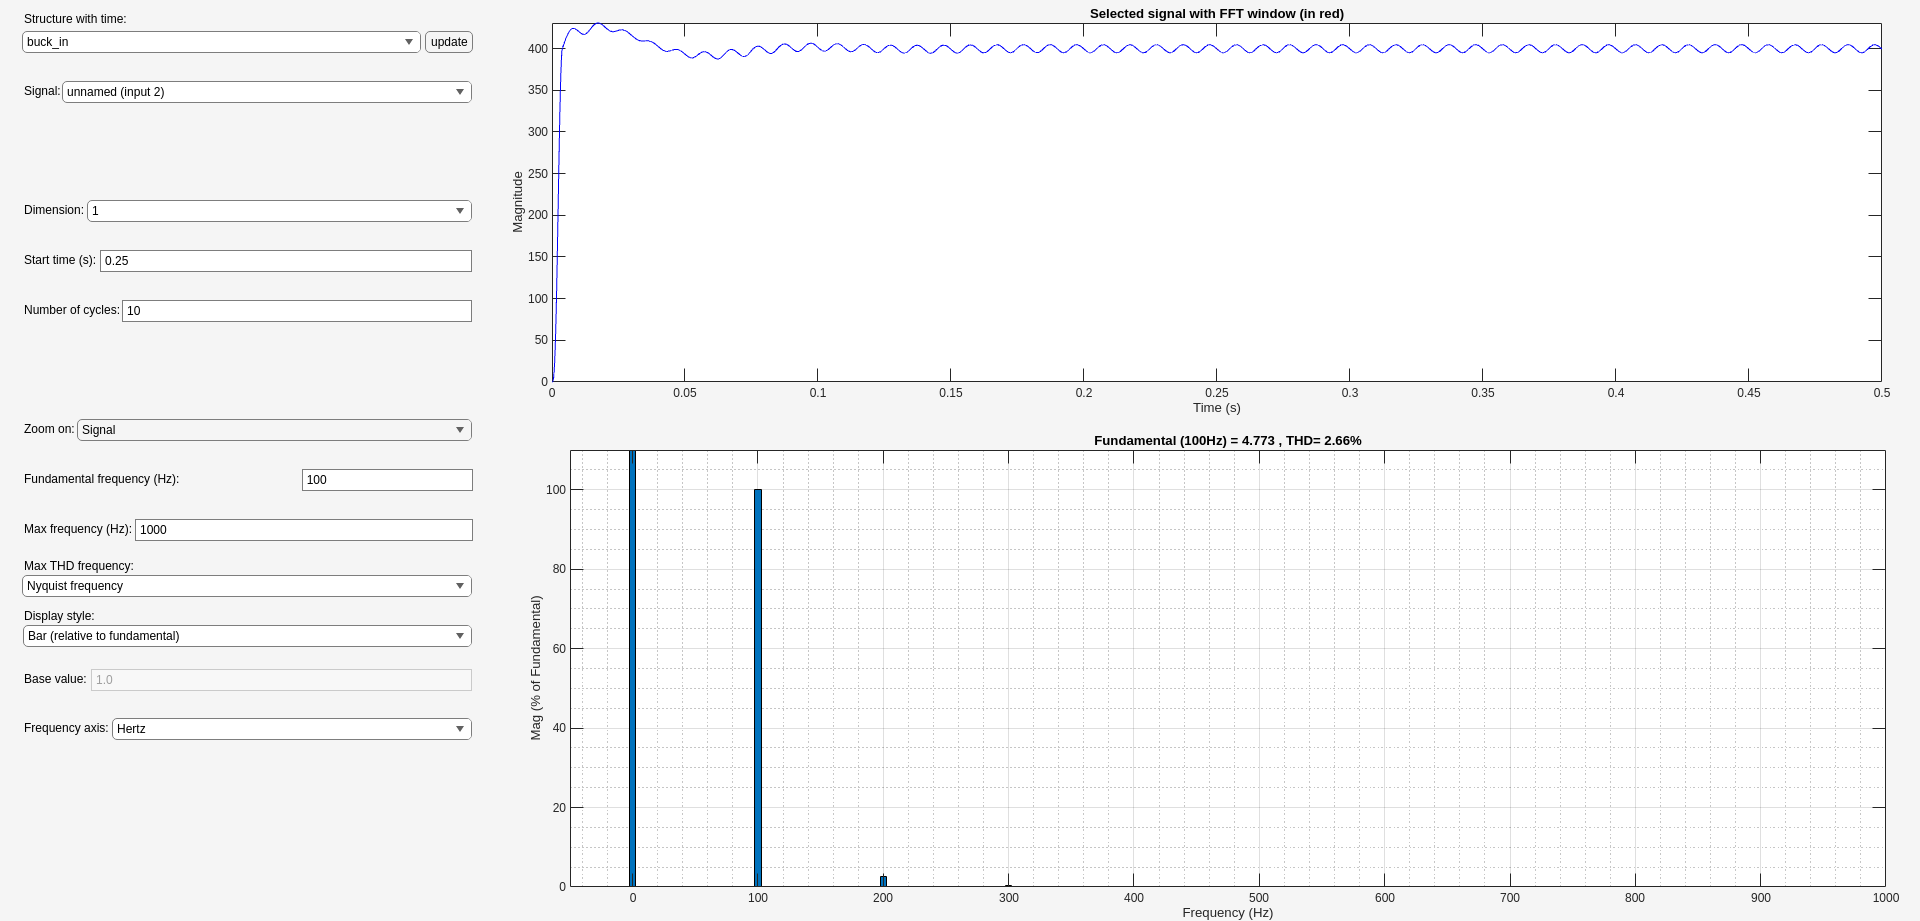
\includegraphics[width=0.8\textwidth]{img/Vout_with_PFC.png}
    \caption{Buck Converter Output with PFC(TDH)}
\end{figure}
\newpage
\section*{References}
\begin{enumerate}
    \item Erickson, R. W., \& Maksimovic, D. (2007). \textit{Fundamentals of Power Electronics} (2nd ed.). Springer.
    \item Texas Instruments. (n.d.). Battery Charger IC Data Sheets. Texas Instruments website. \url{https://www.ti.com}
    \item Mohan, N., Undeland, T. M., \& Robbins, W. P. (2002). \textit{Power Electronics: Converters, Applications, and Design} (3rd ed.). John Wiley \& Sons.
    \item Hart, D. W. (2010). \textit{Power Electronics}. McGraw-Hill Companies Inc., New York.
    \item MathWorks. (n.d.). Power Factor Correction. Retrieved from \url{https://in.mathworks.com/discovery/power-factor-correction.html}
\end{enumerate}

\section*{Future Scope of this Project}
\begin{itemize}
    \item Test other types of PFC methods (using SEPIC PFC, CUK PFC, etc.)
    \item Make the PI values adaptable to the load change.
    \item Use of MOSFET for Full Bridge Rectification.
    \item Use of other efficient techniques to bring down DC voltage.
\end{itemize}

\section*{Acknowledgement}
We sincerely thank IEEE Kerala and BGSW for their invaluable guidance, support, and expertise. This project would not have been possible without their contributions and the resources provided.

\end{document}
